\documentclass[11pt]{article}
\usepackage{listings,amsmath,amssymb,bbm}
\usepackage{amsthm}
\usepackage{graphicx}
\usepackage{color}
\usepackage{multirow}
\usepackage{natbib}
\oddsidemargin0cm
\topmargin-1.4cm
\textheight23.5cm
\textwidth16cm
\parindent0cm
\renewcommand{\baselinestretch}{1.1}
\numberwithin{equation}{section}
\lstset{language=R,basicstyle=\ttfamily\footnotesize,breaklines=true}
\usepackage{booktabs}
\def\R{{\mathbb R}}  %%
\def\N{{\mathbb N}}  %%
\def\E{{\mathbb E}}  %%
\def\Z{{\mathbb Z}}  %%
\def\bc{\boldsymbol{c}}
\def\bd{\boldsymbol{d}}
\def\bx{\boldsymbol{x}}
\def\bm{\boldsymbol{m}}
\def\by{\boldsymbol{y}}
\def\bZ{\boldsymbol{Z}}
\def\bz{\boldsymbol{z}}

\newcounter{saveenumi}
\newcommand{\seti}{\setcounter{saveenumi}{\value{enumi}}}
\newcommand{\conti}{\setcounter{enumi}{\value{saveenumi}}}

\newcommand{\blue}[1]{\textcolor{blue}{#1}}
\newcommand{\red}[1]{\textcolor{red}{#1}}
\usepackage{url}%For ref url
%\bibliographystyle{plain}
%opening
\title{Non-life insurance pricing with gradient tree-boosted mixture models.}
\author{Guangyuan Gao \and Jiahong Li}

\begin{document}

\maketitle

\begin{abstract}
Insurance loss data often cannot be well modeled by a single distribution. Mixture of models are often applied in insurance loss modeling. 
The Expectation-Maximization (EM) algorithm is used for parameter estimation in mixture of models. 
Feature engineering and variable selection are challenging for mixture of models due to several component models involving. 
Overfitting is also a concern when predicting future loss. 
To address those issues, we propose an Expectation-Boosting (EB) algorithm, 
which replaces the maximization step in the EM algorithm by a gradient boosting with decision tree. The boosting is overfitting-sensitive. 
Moreover, it performs automated feature engineering, model fitting and variable selection simultaneously. 
The EB algorithm fully explores the predictive power of covariate space.
We illustrate those advantages in two simulated data and a real insurance loss data.

\end{abstract}

\section{Introduction}

Insurance loss data usually cannot be well modelled by a single distribution.
For claims counts data, there may be an excess of zero claims, so a Poisson distribution is not the best option.
For claims amount data, there may be a heavy tail, so a gamma distribution is not enough to describe the entire data.
One solution to such issues is to apply mixture models.
For claims counts data, we can utilize zero-modified Poisson distribution.
For claims amount data, we can utilize mixture of gamma distribution and heavy-tailed distribution such as Pareto distribution.
When the individual risk factors are available, the mixture of distributions can be extended to mixture of regressions to address the risk heterogeneity in the portfolio.

The Expectation-Maximization (EM) algorithm is an iterative method to estimate component parameters and (hidden) component indicator variable. 
Parameter estimation in mixture models is challenging since component distribution/regression parameters are related to each other. 
Variable selection  is also challenging since we need
to perform variable selection for each component regression.  

\blue{literature review.}

In this paper, we propose an Expectation-Boosting (EB) algorithm, which replaces the maximization step by an overfitting-sensitive boosting step. 
There are several advantages of EB algorithm over the EM algorithm. 
First, boosting algorithm is a flexible non-parametric regression facilitating both non-linear effects and interaction. 
Second, boosting algorithm is overfitting-sensitive, if we add suitable normalization to boosting step (e.g. using decision tree as weak learner) we can perform variable selection simultaneously. 
Third, by investigating the final boosted component, we can select component by removing those components containing very few weak learners. 


Commonly used boosting algorithms are listed below
	\begin{enumerate}
		
		\item Binary classification: {AdaBoost}, LogitBoost (real, discrete, gentle AdaBoost), AdaBoost.M1
		
		\item Multinomial classification: Stagewise Additive Modeling using a Multi-class Exponential loss (SAMME), SAMME.R (multi-class real AdaBoost),
		\item {Gradient based}: {gradient boosting machine/model (GBM)}, Newton boosting, gradient boosting decision tree (GBDT), {eXtreme Gradient Boosting (XGBoost)}, {light gradient boosting machine (LightGBM)}
	\end{enumerate}
	
	The last type is based on {gradient of loss function}, and our EB algorithm uses this version of boosting.

\section{Review: mixture of models and the EM algorithm}


\subsection{Mixture of models}\label{review:mix1}
In this paper, we focus on the exponential distribution family with expectation parameter $\mu$ and dispersion parameter $\phi$. The exponential distribution family is normally sufficient to fit to most insurance loss data.
	Suppose a random variable $y$ follows the $k$-th {\it component distribution} from
	$$\{f_1(y;\mu_1,\phi_1),\ldots,f_K(y;\mu_K,\phi_K)\}$$
	with \textit{mixing probability} $p_k, k=1,\ldots,K$,
	then the probability density function for $y$ is
	$$f(y)=\sum_{k=1}^Kp_kf_k(y;\mu_k,\phi_k).$$

	If {\it individual features $\bx_i$} are available and they have systematic effects on the distribution of $y_i$, then we establish a mixture of regressions:
	$$f(y|\bx)=\sum_{k=1}^Kp_k(\bx)f_k(y;\mu_k(\bx),\phi_k(\bx)).$$
	
	Above is the most general form of mixing. In applications, we always put some constraints on the \textit{mixing structure}:
	
	\begin{itemize}
		\item Mixing probabilities are not related to $\bx$
		$$f(y)=\sum_{k=1}^Kp_kf_k(y;\mu_k(\bx),\phi_k(\bx)).$$
		\item Both mixing probabilities and dispersions are not related to $\bx$
		$$f(y)=\sum_{k=1}^Kp_kf_k(y;\mu_k(\bx),\phi_k),$$

		\item If component distributions are from the same distribution family, we might assume different component distributions have the same dispersion $\phi$
		$$f(y)=\sum_{k=1}^Kp_kf_k(y;\mu_k(\bx),\phi).$$
		\item Covariates $\bx$ are only related to the mixing probabilities:
		$$f(y)=\sum_{k=1}^Kp_k(\bx)f_k(y;\mu_k,\phi_k).$$
	\end{itemize}
	
	We need to determine the mixture structure according to the data and our aim. Imposing suitable constraints on mixture, we can {accelerate model fitting} without compromising predictive performance.

\subsection{EM algorithm}

	Suppose that we know which component distribution $f_k$ each sample $y$ is from. That is we know the \textit{full information} $(Y,\bZ,\bx)$ where
	$$\bZ=(Z_1,\ldots,Z_K)^\top=(\mathbbm{1}_1(k),\ldots,\mathbbm{1}_K(k))^\top$$
	is the one-hot encoding of \textit{component indicator variable}.
	The joint distribution function for full information (one sample) is given by
	$$f(y,\bz|
	\bx) = \prod_{k=1}^K\left[p_k(\bx)f_k(y;\mu_k(\bx),\phi_k(\bx))\right]^{z_k}$$
	The {log-likelihood function} is given by
	\begin{equation}\label{full-L}
		l(p,\mu,\phi|y,\bz,\bx)=\sum_{k=1}^K z_k\left[\log p_k(\bx) + \log f_k(y;\mu_k(\bx),\phi_k(\bx))\right]
	\end{equation}
	Given a data set $(y_i,\bz_i,\bx_i)_{i=1:n}$, the regression coefficients $\theta_p, \theta_\mu, \theta_\phi$ in $p,\mu,\phi$ can be estimated by the following $K+1$ {independent optimizations}
	\begin{equation}\label{p-reg}
		\hat{\theta}_p=\underset{\theta_p}{\arg\max}\sum_{i=1}^n\sum_{k=1}^Kz_{i,k}\log p_k(\bx_i;\theta_p)
	\end{equation}
	\begin{equation}\label{comp-reg}
		\left(\hat{\theta}_\mu^{(k)},\hat{\theta}_\phi^{(k)}\right)=\underset{\theta^{(k)}_\mu,\theta^{(k)}_\phi}{\arg\max}\sum_{i=1}^n\sum_{k=1}^Kz_{i,k}\log f_k\left(y_i;\mu_k\left(\bx_i;\theta_\mu^{(k)}\right),\phi_k\left(\bx_i;\theta_\phi^{(k)}\right)\right), ~\text{for} ~ k=1,\ldots,K.
	\end{equation}
	Those optimizations are corresponding to  {\it a multinomial logistic classification} and {\it $K$ regressions}.
Note that the multinomial logistic classification \eqref{p-reg} are fitted to all samples, while $K$ regressions \eqref{comp-reg} are fitted to {partial} samples with $\{i:z_{i,k}=1\}$.
In practice we do not have full information  $(Y,\bZ,\bx)$ but only the incomplete information $(Y,\bx)$. The following EM algorithm is inspired by the above discussion.
\paragraph{Expectation step.}
	With iterated $\hat{p},\hat{\mu},\hat{\phi}$, calculate the \textit{conditional expectation} of $\bz$:
	$$\hat{z}_{i,k}=\hat{z}_k(\bx_i)=\frac{\hat{p}_{i,k}f_k(y_i;\hat{\mu}_{i,k},\hat{\phi}_{i,k})}{\sum_{l=1}^K\hat{p}_{i,l}f_l(y_i;\hat{\mu}_{i,l},\hat{\phi}_{i,l})},$$
	where
	$\hat{p}_{i,k}=\hat{p}_k(\bx_i)= p_k(\bx_i;\hat{\theta}_p),\hat{\mu}_{i,k}=\hat{\mu}_k(\bx_i)=\mu_k\left(\bx_i;\hat{\theta}_\mu^{(k)}\right),\hat{\phi}_{i,k}=\hat{\phi}_k(\bx_i)=\phi_k\left(\bx_i;\hat{\theta}_\phi^{(k)}\right)$.

\paragraph{Maximization step.}
	Based on the following likelihood function for full information, calculate the MLE of regression coefficients  $\theta_p, \theta_\mu, \theta_\phi$.
	\begin{equation}
		\begin{aligned}
			&l(p,\mu,\phi|y,\hat{z},\bx)\\
			=&\sum_{i=1}^n\sum_{k=1}^K \hat{z}_{i,k}\left[\log p_k(\bx_i;\theta_p) + \log f_k\left(y_i;\mu_k\left(\bx_i;\theta_\mu^{(k)}\right),\phi_k\left(\bx_i;\theta_\phi^{(k)}\right)\right)\right]\\
			=&\sum_{i=1}^n\sum_{k=1}^K \hat{z}_{i,k}\log p_k(\bx_i;\theta_p) + \sum_{i=1}^n\sum_{k=1}^K \hat{z}_{i,k}\log f_k\left(y_i;\mu_k\left(\bx_i;\theta_\mu^{(k)}\right),\phi_k\left(\bx_i;\theta_\phi^{(k)}\right)\right)
		\end{aligned}
	\end{equation}
	This step is similar to \eqref{p-reg} and \eqref{comp-reg}. However, now we have $\hat{z}_{i,k}\in(0,1)$, 
	so we need to consider a multinomial logistic classification with {fractional} response and $K$ {weighted}-regressions fitted to {all} samples.

\section{Expectation-Boosting algorithm}
We replace the maximization step in the EM algorithm by a boosting step. The boosting step increases the likelihood in each iteration, but overfitting-sensitively.
The boosting step follows a generic functional gradient descent algorithm.
We first review generic functional gradient descent algorithm, then describe our proposed EB algorithm.

\subsection{Generic functional gradient descent algorithm}

	Suppose a {non-parametric regression function} as $F:\R^P\rightarrow\R$. Our purpose is to  estimate $F$ to minimize the expected loss $$\hat{F}=\underset{F}{\arg\min}\E\left[C(Y,F(\bx))\right],$$
	where $C:\R\times\R\rightarrow\R_+$ is the \textit{loss function}.
	We always replace the expected loss by sample average loss:
	$$\hat{F}=\underset{F}{\arg\min} \frac{1}{n}\sum_{i=1}^nC(y_i,F(\bx_i))$$
	We choose the \textit{negative log-likelihood} function as the loss function. Hence, minimizing the loss function is equivalent to maximizing the likelihood function.
The link function is used to link the regression function $F$ with the parameter interested such as mean, probability odds, etc. 
	Commonly used {link function} and loss functions in different boosting algorithms are listed below:
	\begin{itemize}
		\item AdaBoost: $$C(y,F)=\exp(yF),  ~~ y\in\{-1,1\}$$
		$$F(\bx)=\frac{1}{2}\log\left(\frac{\Pr[Y=1|\bx]}{\Pr[Y=-1|\bx]}\right)$$
		\item LogitBoost: $$C(y,F)=\log_2(1+\exp(-2yF)), ~~ y\in\{-1,1\}$$
		$$F(\bx)=\frac{1}{2}\log\left(\frac{\Pr[Y=1|\bx]}{\Pr[Y=-1|\bx]}\right)$$
		\item $L_2$Boost: 
		\begin{equation}\label{l2}
			C(y,F)=(y-F)^2/2, ~~ y\in \R
		\end{equation}
		$$F(\bx)=\E(Y|\bx)$$
	\end{itemize}

We follow \citet{buehlmann:2003} to review the generic functional gradient decent algorithm:

	\begin{enumerate}
		\item Initialization: $\hat{F}^{[0]}(\bx;\hat{\theta}^{[0]}),$ where $\hat{\theta}^{[0]}$ are determined by $(y_i,\bx_i)_{i=1:n}$.
		Let $m=0.$
		\item Projection of gradient to weak learner:
		Calculate \textit{negative gradient} $$u_i=\left.-\frac{\partial C(y_i,F)}{\partial F}\middle|_{F=\hat{F}^{[m]}(\bx_i)}\right., i=1,\ldots,n.$$
		Data $(u_i,\bx_i)_{i=1:n}$ is used to calibrate a weak learner $\hat{f}^{[m+1]}(\bx;\hat{\theta}^{[m+1]})$ with \textit{loss function $L_2$} \eqref{l2}.
	
		\item One-dimensional optimization:
		Solve an one-dimensional optimization  to find \textit{expansion coefficient} $\hat{\omega}^{[m+1]}$:
		$$\hat{\omega}^{[m+1]}=\underset{\omega}{\arg\min}\sum_{i=1}^n C(y_i, \hat{F}^{[m]}(\bx_i)+\omega\hat{f}^{[m+1]}(\bx_i))$$
		Update $$\hat{F}^{[m+1]}=\hat{F}^{[m]}+s\hat{\omega}^{[m+1]}\hat{f}^{[m+1]},$$
		where $s$ is \textit{shrinkage factor} (learning rate).
		\item Iteration: Let $m$ increase by 1, and repeat steps 2-3.
			\end{enumerate}
In the algorithm, weak learners are fitted to negative gradient $U$ rather than $Y$.
		 Loss function in weak learners is always $L_2$, independently with model loss function $C$. 
		 If weak learners are trees, the algorithm is called \textit{gradient boosting decision tree (GBDT)}, and {calibration and variable selection} are performed simultaneously.
		\citet{buhlmann2007boosting} argue that step 3 of one-dimensional optimization seems unnecessary given learning rate $s$ is sufficiently small according to some empirical experiments.




\subsection{Expectation-Boosting algorithm}

We denote the regression functions for the interested parameters $p,\mu,\phi$ by {$F,G,H$}. In the EB algorithm, we need to specify link functions and cost/loss functions, which determines negative gradient function.
For mixing probabilities $p$, we choose multiple logistic link function for mixing probabilities.	
	\begin{equation}\label{logistic}
		p_k(F(\bx))=\Pr(Z_k=1|\bx)=\frac{\exp{F_k(\bx)}}{\sum_{l=1}^{K}\exp{F_l(\bx)}},
	\end{equation}
	or equivalently
	\begin{equation}\label{inv-logistic}
		F_k(\bx)=\log p_k(\bx)-\frac{1}{K}\sum_{l=1}^K\log p_l(\bx),~~k=1,\ldots,K.
	\end{equation}
We use the negative log-likelihood function as the cost function
\begin{equation}
	\begin{aligned}
		{C_{Z}(\bZ, F(\bx))}=& - \sum_{k=1}^K Z_k \log p_k(\bx).
	\end{aligned}
\end{equation}
The negative gradient of the cost function w.r.t. $F_k$ is given by
\begin{equation}
	{U_k(\bZ,F(\bx))}=-\frac{\partial C_{Z}(\bZ,F(\bx))}{\partial F_k(\bx)}=
	Z_k-p_k(\bx), ~~k=1,\ldots,K
\end{equation}

For component parameters $\mu$ and $\phi$, the link function and cost function (distribution) depend on the loss data.
Commonly used link functions in component models are indicated as follows
	\begin{itemize}
		\item Component Gaussian model:
		$$\mu_k(G_k(\bx))=G_k(\bx)$$
		$$\phi_k(H_k(\bx))=\exp H_k(\bx)$$
		\item Component Poisson model:
		$$\mu_k(G_k(\bx))=\exp G_k(\bx)$$
		\item Component gamma model:
		$$\mu_k(G_k(\bx))=\exp G_k(\bx)$$
		$$\phi_k(H_k(\bx))=\exp H_k(\bx)$$
	\end{itemize}
Note that we slightly abuse function notations $p_k,\mu_k,\phi_k$ (i.e. the inverse link function); in Section \eqref{review:mix1} they define different functions.
The negative log-likelihood function of each component model is used as its cost function:
	\begin{equation}
		\begin{aligned}
			{C_k(Y,\bZ,G_k(\bx))}=& -Z_k\log f_k(Y;\mu_k(G_k(\bx)),\phi_k), ~ k=1:K.
		\end{aligned}
	\end{equation}
	The negative gradient of $C_k$ w.r.t. $G_k$ is given by 
	$${V_k(Y,\bZ,G_k(\bx))}=-\frac{\partial C_k(Y,\bZ,G_k(\bx))}{\partial G_k(\bx)}.$$
	Note that we have assumed that dispersion $\phi_k$ is fixed among samples (not related to $\bx$) to avoid lengthy notations. The extension to dispersion modelling is straightforward; please refer to the real data analysis in Section ??.

Upon the above defined notations, we are ready to introduce the proposed EB algorithm.
We first summarize the proposed EB algorithm as follows, then we detail each step.
\begin{enumerate}
	\item[1] Initialization of EB algorithm $\hat{p}^{[0]},\hat{\mu}^{[0]},\hat{\phi}^{[0]}$. Set $t=0$.
	
	\item[2] Calculating conditional expectation of latent variable $\hat{z}^{[t]}$ given $\hat{p}^{[t]},\hat{\mu}^{[t]},\hat{\phi}^{[t]}$.
	
	\item[3.1]  Gradient boosting mixing probabilities $\hat{p}^{[t+1]}$  given latent variable $\hat{z}^{[t]}$.
	\item[3.2] Gradient boosting component model parameters $\hat{\mu}^{[t+1]}$ given latent variable $\hat{z}^{[t]}$.
	\item[4]  Calculate the MLE $\hat{\phi}^{[t+1]}$. Increase $t$ by 1. Repeat steps 2-3 until $t$ reaches to $T$.
	
\end{enumerate}
Note that we can perform steps 3.1 and 3.2 simultaneously by parallel computing which dramatically save running time.  Also note that  in the algorithm we have assumed that dispersion $\phi_k$ is fixed among samples (not related to $\bx$). The extension to dispersion modelling is straightforward by adding another gradient boosting step 3.3 for component model parameter $\phi$ and removing the MLE calculation in step 4.
	
In step 1 of initialization of EB algorithm, we neeed to initialize the following quantities.
	\begin{enumerate}
		\item[1.1] Initialize $\hat{p}_1^{[0]}, \ldots,\hat{p}_K^{[0]}$ and   $\hat{F}_1^{[0]}, \ldots, \hat{F}_{K}^{[0]}$:
		
		\begin{itemize}
			\item 	$\hat{p}_k^{[0]}=\frac{1}{K}$
			\item $\hat{F}_1^{[0]}, \ldots, \hat{F}_{K}^{[0]}$ are obtained by \eqref{inv-logistic}.
		\end{itemize}
		\item[1.2]
		Initialize $\hat{\mu}_1^{[0]},\ldots,\hat{\mu}_K^{[0]}$ and  $\hat{G}_1^{[0]},\ldots,\hat{G}_K^{[0]}$:
		
		\begin{itemize}
			\item $\hat{\mu}_k^{[0]}=\frac{\sum_{i=1}^nY_i}{n}$
			\item $\hat{G}_k^{[0]}=\mu_k^{-1}(\hat{\mu}_k^{[0]})$
		\end{itemize}
		\item[1.3] Initialize $\hat{\phi}_1^{[0]},\ldots, \hat{\phi}_K^{[0]}$ as the sample variance. (Assume that dispersion is independent with covariates.)
		\item[1.4] 	Set $t=0$.
	\end{enumerate}
	

In step 2 of conditional expectation of latent variable, we set  $\hat{z}_{i,k}^{[t]}$ as
	\begin{equation*}
		\hat{z}_{i,k}^{[t]}=\frac{\hat{p}_{k}^{[t]}(\bx_i) f_{k}\left(y_i ; \hat{\mu}_{k}^{[t]}(\bx_i), \phi_k^{[t]} \right)}{\sum_{l=1}^{K} \hat{p}_{l}^{[t]}(\bx_i) f_{l}\left(y_i ; \hat{\mu}_{l}^{[t]}(\bx_i), \phi_l^{[t]}\right)},~~ k=1:K.
	\end{equation*}


In step 3.1 of gradient boosting mixing probabilities, we implement a  multinomial logistic classification boosting with fractional response: 
	\begin{enumerate}
		\item[3.1.1] Initialization. Set $\hat{p}_1^{[t,0]}, \ldots, \hat{p}_K^{[t,0]}$ and $\hat{F}_1^{[t,0]}, \ldots, \hat{F}_{K}^{[t,0]}$ as
		\begin{equation}\label{ini-1}			
		\hat{p}_k^{[t,0]}=\frac{1}{K},
		~~\hat{F}_k(\bx)^{[t,0]}=\log \hat{p}_k^{[t,0]}-\frac{1}{K}\sum_{l=1}^K\log \hat{p}_l^{[t,0]}
	\end{equation}
		Set $m=0$.
		\item[3.1.2] Projection of gradient to learner.
		Compute the negative gradient sample $u_{1,k}^{[t,m]},\ldots,u_{n,k}^{[t,m]}$,  in which
		$$u_{i,k}^{[t,m]}=U_k(\hat{\bz}_{i}^{[t]},\hat{F}^{[t,m]}(\bx_i))=\hat{z}_{i,k}^{[t]}-\hat{p}_{i,k}^{[t,m]}.$$
		For each $k$, the data $(u_{i,k}^{[t,m]},\bx_i)_{i=1:n}$ is used to calibrate a $L$-terminal node regression trees $\hat{f}_k^{[t,m+1]}\left(\bx;R^{[t,m+1]}_{l=1:L},\bar{u}^{[t,m+1]}_{l=1:L}\right)$ with $L_2$ loss,
		where $R^{[t,m+1]}_{l=1:L}$ is the partition of covariate space and $\bar{u}^{[t,m+1]}_{l=1:L}$ contains the average gradient in each terminal node.
		
		
	
		\item[3.1.3]  The one-dimensional optimization for expansion coefficient leads to the following update \citep{friedman2001greedy}:
		
		$$\hat{F}_k^{[t,m+1]}(\bx_i)=\hat{F}_k^{[t,m]}(\bx_i)+s\sum_{l=1}^L\gamma^{[t,m+1]}_l\mathbbm{1}(\bx\in R^{[t,m+1]}_l),~ k=1,\ldots,K$$
		where
		$$\gamma^{[t,m+1]}_l=\frac{K-1}{K}\frac{\sum_{\bx_i\in R_l^{[t,m+1]}}u_{i,k}^{[t,m]}}{\sum_{\bx_i\in R_l^{[t,m+1]}}|u_{i,k}^{[t,m]}|(1-|u_{i,k}^{[t,m]}|)}$$
		We then derive the updated mixing probability $\hat{p}^{[t,m+1]}_{k=1:K}$  using \eqref{logistic}.
		
		
	
		\item[3.1.4] Increase $m$ by 1, and repeat steps 3.1.2-3.1.3  until $m$ reaches to the pre-determined $M_p$.
		Set $$\hat{F}_k^{[t+1]}=\hat{F}_k^{[t,M_p]},~~\hat{p}_k^{[t+1]}=\hat{p}_k^{[t,M_p]},$$
	\end{enumerate}
Note that  $K$ regression trees are fitted independently in step 3.1.2. We can accelerate this step by parallel computing.

In step 3.2 of gradient boosting component models, we implement $K$ weighted boosting:
	\begin{enumerate}
		\item[3.2.1] Initialization. Set $\hat{\mu}_1^{[t,0]},\ldots,\hat{\mu}_K^{[t,0]}$ and $\hat{G}_1^{[t,0]},\ldots,\hat{G}_K^{[t,0]}$:
			\begin{equation}\label{ini-2}
				\hat{\mu}_k^{[t,0]}=\frac{\sum_{i=1}^nY_i}{n}, \hat{G}_k^{[t,0]}=\mu_k^{-1}(\hat{\mu}_k^{[t,0]}).
			\end{equation}
		
		Set $m=0$.
		\item[3.2.2] Projection of gradient to learner.
		Compute the negative gradient samples $v_{1,k}^{[t,m]},\ldots,v_{n,k}^{[t,m]}$, in which
		$$v_{i,k}^{[t,m]}=V_k(y_i,\hat{\bz}^{[t]}_{i},\hat{G}^{[t,m]}(\bx_i)),$$
		For each $k$, the data $(v_{i,k}^{[t,m]},\bx_i)_{i=1:n}$ is used to calibrate a $L$-terminal node regression trees $\hat{g}_k^{[t,m+1]}\left(\bx;S^{[t,m+1]}_{l=1:L},\bar{v}^{[t,m+1]}_{l=1:L}\right)$ with $L_2$ loss, where $S^{[t,m+1]}_{l=1:L}$ is the partition of covariate space and $\bar{v}^{[t,m+1]}_{l=1:L}$ contains the average gradient in each terminal node.
		
	
	
		\item[3.2.3]  Conduct the following $K$ independent one-dimensional optimizations to find the best expansion coefficients.
		$$\hat{w}_{k}^{[t,m+1]}=\underset{w}{\arg\min}\sum_{i=1}^n C_{k}(y_i,\hat{\bz}_i^{[t]},\hat{G}_k^{[t,m]}(\bx_i)+w\hat{g}_k^{[t,m+1]}(\bx_i)).$$
		
		\item[3.2.4]  For each $k$, compute the updates
		$$\hat{G}_k^{[t,m+1]}(\bx_i)=\hat{G}_k^{[t,m]}(\bx_i)+s\hat{w}_{k}^{[t,m+1]}\hat{g}_{k}^{[t,m+1]}(\bx_i),$$
		$$\hat{\mu}_k^{[t,m+1]}(\bx_i)=\mu_k(\hat{G}_k^{[t,m+1]}(\bx_i)).$$
		\seti


		\item[3.2.5] Increase $m$ by 1, and repeat steps 3.2.2-3.2.4 until $m$ reaches to the pre-determined $M_\mu$. Set
		$$\hat{G}_k^{[t+1]}=\hat{G}_k^{[t,M_\mu]},~~\hat{\mu}_k^{[t+1]}=\hat{\mu}_k^{[t,M_\mu]}.$$
	\end{enumerate}
Note that $K$ independent boosting are implemented in step 3.2, we can accelerate this step by parallel computing.
	
In step 4, 
%for parameters not related to covariate $\bx$, 
compute the MLE $\hat{\phi}_k^{[t+1]}$ given all the other parameters $\hat{p}_k^{[t+1]}, \hat{\mu}_k^{[t+1]}$, then increase $t$ by 1 and repeat steps 2-3 until $t$
		reaches to the pre-determined $T$.
		
In the EB algorithm, we have the following tuning parameters and the corresponding tuning strategies are listed below:
	\begin{itemize}
		\item Number of EB iterations {$T$} (iterations in outer loop). This can be determined by screening the trace plot of loss.
		\item Number of iterations in boosting {$M_p,M_\mu$} (iterations in inner loops). We can specify a sufficiently large $M_p,M_\mu$ and use  early stop according to validation loss.
		\item Learning rate {$s$}. Smaller learning rate tends to lead to a better fitting and predictive performance but requiring more inner iterations.
		\item Tuning parameters in base learner tree: complexity parameter, maximum depth, number of terminal nodes. Those parameters can be tuned as in typical decision trees.
	\end{itemize}

		
{\bf Remarks.}
	In initialization of boosting steps 3.1.1 and 3.2.1, we initialize parameters {independently} with the previously boosting estimates $\hat{p}_k^{[t-1]}, \hat{\mu}_k^{[t-1]}$; see equations \eqref{ini-1} and \eqref{ini-2}. We call this as independent boosting.
	In contrast, we might initialize parameters as the previously boosted estimates $$\hat{p}_k^{[t,0]}=\hat{p}_k^{[t-1]}, \hat{\mu}_k^{[t,0]}=\hat{\mu}_k^{[t-1]}.$$
		This would lead a {smaller} required inner boosting iterations $M$ (or a {earlier} stop on validation loss). 
	We call this as forward boosting. 
	However, with forward boosting, it is difficult to predict for new data due to the {iterative initialization}. One solution is to apply an additional boosting with default initialization \eqref{ini-1} and \eqref{ini-2} given the {last expected hidden variables $\hat{\bz}_i^{[T]}$}. In the following applications, we only implement independent boosting.
			
\section{Applications}

We conduct two simulated data analysis and a real data analysis. 
The first simulated data follows a mixture of Gaussian models. 
We use this example to illustrate the advantages of the EB algorithm over the EM algorithm.
The second simulated data follows a zero-inflated Poisson model, which mimics claims counts data with excess of zero.
The real data contains the claims severity of an insurance company. This example demonstrates how we choose component models and mixing structure in practice.



\subsection{First simulated example: mixture of Gaussians}

\red{I want to use three gaussians example in this part, and follows the  structure below.}

The underlying model is specified as follows:
	$$Y_i =Z_iY_{i,1}+(1-Z_i)Y_{i,2}$$
	$$Y_{i,1}|\bx_i \sim N(\mu_1(\bx_i), 0.9^2)$$
	$$Y_{i,2}|\bx_i \sim N(\mu_2(\bx_i), 0.5^2)$$
	$$Z_i \sim Bernuli(p(\bx_i))$$
	$$\bx_i=(x_{i,1},x_{i,2},x_{i,3})^{\top}$$
	$$\mu_1(\bx_i)=2+2\times x_{i,1} + \log x_{i,2}$$
	$$\mu_2(\bx_i) = 0.5-0.5\times x_{i,1}+x_{i,3}-x_{i,1}\times x_{i,2}$$
	$$p(\bx_i)=\frac{\exp\eta(\bx_i)}{1+\exp\eta(\bx_i)}$$
	$$\eta(\bx_i)=1+0.1\times x_1+\log x_2 +x_3\times x_1$$
The covariate is generated from the following distribution:
	$$x_{1,i}\sim N(2,1^2)$$
	$$x_{i,2}\sim Exp(2)$$
	$$x_{i,3}\sim Bernuli(0.5)$$
We simulate $n=5,000$ observations, Figure \ref{norm-hist-y} shows the empirical distribution of $ZY,(1-Z)Y,Y$.
	\begin{figure}[htp!]
		\centering
		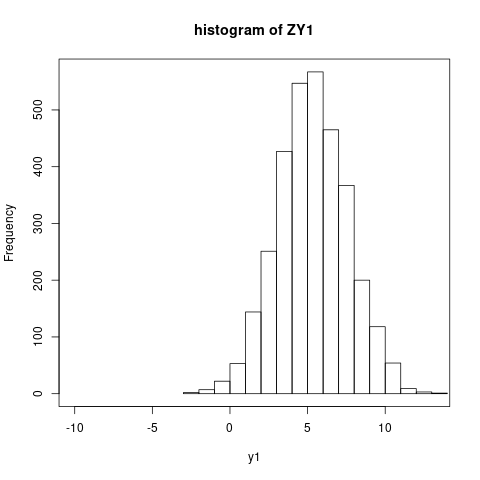
\includegraphics[width=0.3\linewidth]{../plots/two_gaussians/yone}
		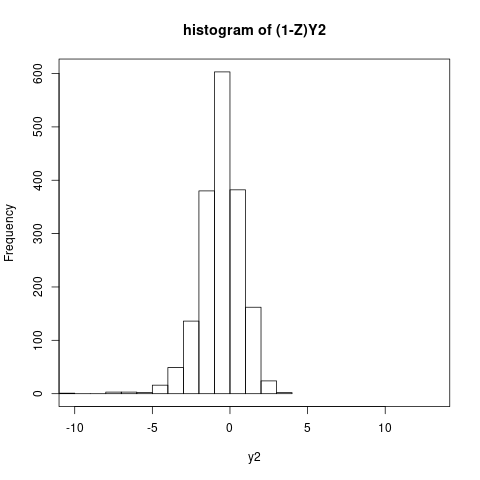
\includegraphics[width=0.3\linewidth]{../plots/two_gaussians/ytwo}
		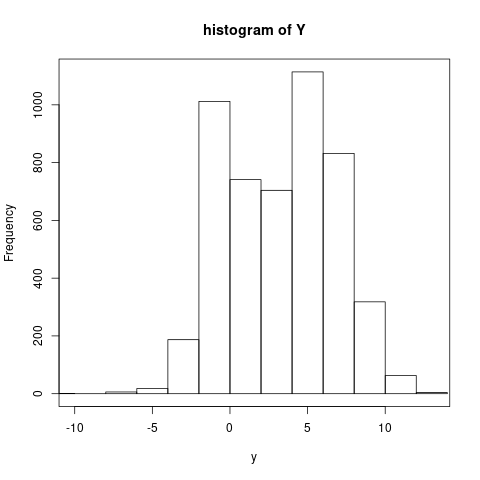
\includegraphics[width=0.3\linewidth]{../plots/two_gaussians/y}
		\caption{Distribution of $ZY,(1-Z)Y,Y$.}\label{norm-hist-y}
	\end{figure}
We fit the following 5 models:
\begin{itemize}
	\item 	Mixture of distributions (homo):
	$$f(y;p,\mu,\sigma)=p_1f_N(y;\mu_1,\sigma_1^2)+(1-p_1)f_N(y;\mu_2,\sigma_2^2)$$
	\item 	Mixture of linear regressions or mixture of boosting with {constant} mixing probabilities (glm\_cp or boosting\_cp)
	$$f(y;p,\mu,\sigma)=p_1f_N(y;\mu_1(\bx),\sigma_1^2)+(1-p_1)f_N(y;\mu_2(\bx),\sigma_2^2)$$
	\item 	Mixture of linear regressions or mixture of boosting with {varying} mixing probabilities (glm\_vp or boosting\_vp)
	$$f(y;p,\mu,\sigma)=p_1(\bx)f_N(y;\mu_1(\bx),\sigma_1^2)+(1-p_1(\bx))f_N(y;\mu_2(\bx),\sigma_2^2)$$
\end{itemize}
We summarize the test losses in Table \ref{gaussian-summary}. Note that we have defined three metrics based on the true parameters: 
	$$e_{\mu 1}=\frac{\sum_{i=1}^{n}(\mu_{i,1}-\hat{\mu}_{i,1})^2}{n}$$
	$$e_{\mu 2}=\frac{\sum_{i=1}^{n}(\mu_{i,2}-\hat{\mu}_{i,2})^2}{n}$$
	$$e_{\eta}=\frac{\sum_{i=1}^{n}(\eta_{i}-\hat{\eta}_{i})^2}{n},$$
	where $\eta_i=\log\frac{p_i}{1-p_i}$.
	\begin{table}[htp!]
		\centering
		\caption{Summary of test losses for different models.}\label{gaussian-summary}
		\begin{tabular}{c|rrrr}
			\hline
			model        & \multicolumn{1}{c}{neg LL} & \multicolumn{1}{c}{$e_{\mu 1}$} & \multicolumn{1}{c}{$e_{\mu 2}$} & \multicolumn{1}{c}{$e_{\eta}$} \\ \hline
			homo         & 2.5868                   & 6.2657                         & 2.6688                        & 3.3304                             \\
			glm\_cp      & 1.8978                   & 0.7775                         & 0.3233                         & 3.2440                             \\
			glm\_vp      & 1.7698                   & 0.8028                         & 0.3260                         & 1.2667                             \\
			boosting\_cp & 1.7492                   & 0.2461                         & {\bf 0.1062}                        & 3.2242                             \\
			boosting\_vp & {\bf 1.6407}                  & {\bf 0.2334}                         & 0.1105                         & {\bf 0.8435}                             \\ \hline
		\end{tabular}
	\end{table}
Hence, we see the mixture of boosting with varying mixing probabilities has the outstanding out-of-sample predictive performance.

\red{Accelerating by paralleling computing}


\subsection{Second simulated example: zero-inflated Poisson model}

We consider another simulated data which is generated from a zero-inflated Poisson (ZIP) model. This simulated example mimics number of claims which usually involves excess of zero claims compared with a fitted Poisson distribution.
The underlying  model is given as follows:
 \begin{equation}
	f_{\text{ZIP}}(N;\lambda,\pi_0) = \left\{ 
	\begin{array}{ccl}
		\pi_0+(1-\pi_0)e^{-\lambda} & \mbox{for}
		& N=0 \\
		(1-\pi_0)\frac{e^{-\lambda}\lambda^N}{N!} & \mbox{for} &N\in\N_+.
	\end{array}\right.
\end{equation}
The ZIP model is a mixture of a probability mass of 1 at 0 and a Poisson distribution. The mixing probability is $\pi_0$ and $1-\pi_0$.
The probability density function can be written as
$$f_\text{ZIP}(N;\lambda,\pi_0)= \pi_0\mathbbm{1}_{\{N=0\}} + 
(1-\pi_0)\frac{e^{-\lambda}\lambda^N}{N!}.$$
Five covariates $\bx=(x_1,\ldots,x_5)^\top$ have systematic effects on both $\pi_0$ and $\lambda$ as follows:
\begin{equation}
	\pi_0(\bx)=\frac{\exp F(\bx)}{1+\exp F(\bx)}, ~~
	\lambda(\bx)=\exp G(\bx), 
\end{equation}
where
\begin{equation}
	 F(\bx)=0.3-2x_2^2+x_2+0.2x_5, ~~G(\bx)=\log 0.5+x_1^2 + 0.2\log x_3 - 0.2x_1 x_4.
\end{equation}
The covariates are generated from the following distributions:
$$	x_1~\sim~N(0,0.5^2), ~~ x_2~\sim~U(0,1), ~~ x_3~\sim~\Gamma(2,0.5),$$ $$x_4~\sim~Bernulli(0.5),~~ x_5~\sim~Bernulli(0.2).$$
Note that we use shape-rate parameters for gamma distribution.



\subsection{A real data example: claims severity modelling}
		
\begin{frame}{Distribution of average claim amount}
	Claims amount data {\tt freMTPL2sev} from R package {\bf CASdatasets}. Sample size $n=24,938$. \blue{Three peaks and heavy tail}.
	\begin{figure}[h!]
		\centering
		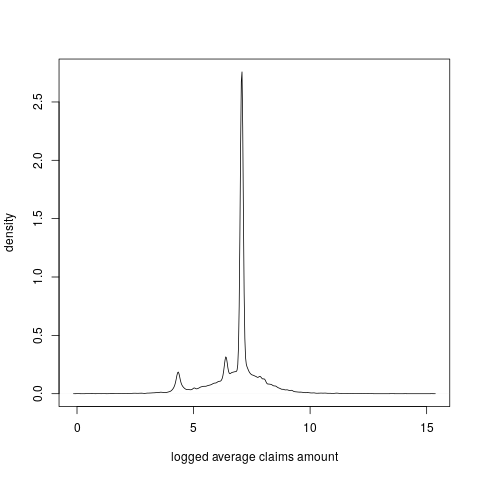
\includegraphics[width=0.35\linewidth]{../plots/sev/hist.png}
		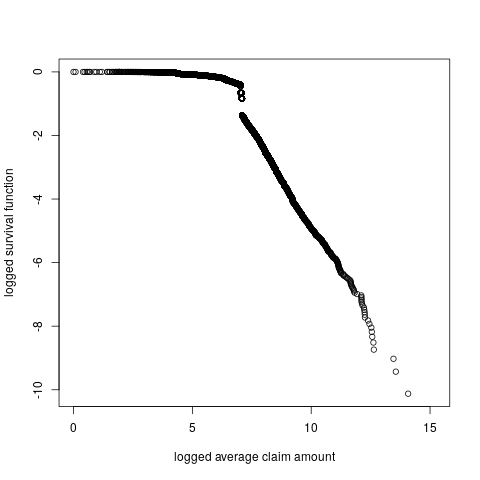
\includegraphics[width=0.35\linewidth]{../plots/sev/log-log.png}
		\caption{Histogram and logged survival function of logged average claims.}\label{tail}
	\end{figure}
\end{frame}

\begin{frame}{Mixture of distributions}
	Three gamma distributions for three peaks. One gamma distribution for resting non-tail part. One Pareto distribution for tail.
	$$f(y)=\sum_{k=1}^4p_kf_{gamma}(y;\mu_k,\phi_k)+p_5f_{pareto}(y;\alpha,M)$$
	where $\mu,\phi$ are mean and dispersion parameter, and $\alpha, M$ are tail index and threshold. The threshold is pre-determined as $8158.13$ according to Hill plot.
\end{frame}

\begin{frame}{Initialization of hidden variable}
	
	Figure \ref{tail} indicates a way to initialize the hidden variable:
	\begin{equation}
		\begin{aligned}
			\hat{z}^{[0]}_i&=(\hat{z}^{[0]}_{i,1},\hat{z}^{[0]}_{i,2},\hat{z}^{[0]}_{i,3},\hat{z}^{[0]}_{i,4},\hat{z}^{[0]}_{i,5})^\top\\
			&=(\mathbbm{1}_{(0,500]}y_i,\mathbbm{1}_{(500, 1000]}y_i,\mathbbm{1}_{(1000,1200]}y_i,\mathbbm{1}_{(1200,8158.13]}y_i,\mathbbm{1}_{(8158.13,\infty)}y_i)^\top
		\end{aligned}
	\end{equation}
	
	Other parameters can be initialized as the MLE based on the full likelihood function.
	
\end{frame}


\begin{frame}{EM algorithm}
	\begin{figure}[h!]
		\centering
		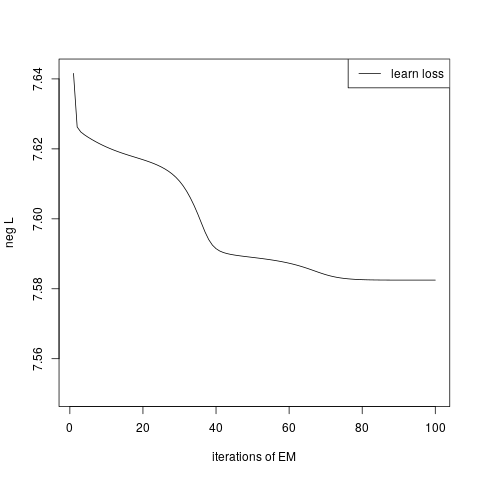
\includegraphics[width=0.35\linewidth]{../plots/sev/null_trace}
		\caption{Learning loss of mixture of distributions.}\label{null_sev}
	\end{figure}
\end{frame}

\begin{frame}{Estimated parameters}	\begin{table}[h!]
		\centering
		\caption{MLE of four component gamma distributions. Tail index is estimated as $\hat{\alpha}=1.0773$}\label{null-gamma}
		\begin{tabular}{crrrr}
			\hline
			component $k$ & \multicolumn{1}{c}{$\mu_k$} & \multicolumn{1}{c}{shape $(1/\phi_k)$} & \multicolumn{1}{c}{scale} & \multicolumn{1}{c}{rate} \\ \hline
			1         & 76.8727                & 105.556                   & 0.7283                    & 1.3731                   \\
			2         & 592.5909               & 653.539                   & 0.9067                    & 1.1029                   \\
			3         & 1171.3811              & 999.9999                  & 1.1714                    & 0.8537                   \\
			4         & 1534.5143              & 1.0377                    & 1478.7768                 & 7e-04                    \\ \hline
		\end{tabular}
	\end{table}
	
	~
	
	Those large shape parameters (small dispersion) implies the difficulties with \blue{gamma mean modeling}.
\end{frame}

\begin{frame}{Boosting mixing probabilities}
	$$f(y|\bx)=\sum_{k=1}^4p_k(\bx)f_{gamma}(y;\mu_k,\phi_k)+p_5(\bx)f_{pareto}(y;\alpha,M)$$
	\begin{figure}[htp!]
		\centering
		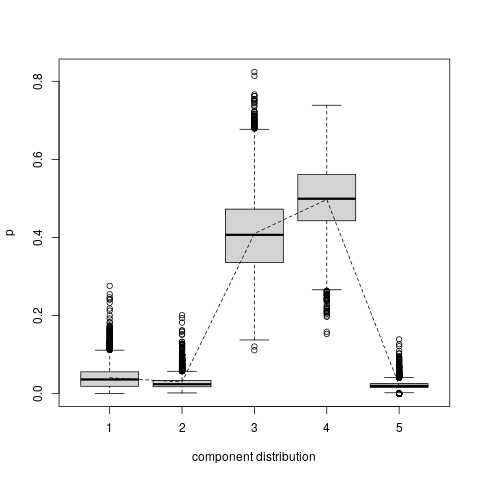
\includegraphics[width=0.35\linewidth]{../plots/sev/glm_p}
		\caption{Boxplot of estimated mixing probabilities.}\label{glm-p}
	\end{figure}
\end{frame}

\begin{frame}{Boosting the forth component  mean}
	$$
	\begin{aligned}
		f(y|\bx)=&\sum_{k=1}^3p_k(\bx)f_{gamma}(y;\mu_k,\phi_k)+ \\
		&p_4(\bx)f_{gamma}(y;\mu_4(\bx),\phi_4)+ p_5(\bx)f_{pareto}(y;\alpha,M)
	\end{aligned}
	$$
	Test loss (negative log-likelihood)
	\begin{enumerate}
		\item Mixture of distributions:
		7.5815
		\item Boosting mixing probabilities:
		{\bf 7.5588}
		\item Boosting mixing probabilities and the forth component mean:
		7.5573.
	\end{enumerate}
\end{frame}

\section{Conclusions}
\begin{frame}{Our proposal: Expectation-Boosting algorithm}
	Expectation-Boosting (EB) algorithm:
	\begin{itemize}
		\item Replaces the maximization step by an \blue{overfitting-sensitive} boosting step.
		\item The boosting step follows a \blue{generic functional gradient descent algorithm}.
		
	\end{itemize}
\end{frame}

\begin{frame}{Advantages}
	Several advantages of EB algorithm over the EM algorithm.
	\begin{itemize}
		\item No need for specifying the form of component regression functions and performing covariate transformation.
		\item Only need for component \blue{loss functions}.
		\item Boosting algorithm is a flexible non-parametric regression facilitating both \blue{non-linear effects and interaction}.
		\item  Boosting algorithm is \blue{overfitting-sensitive}, we can perform \blue{variable selection} simultaneously during the EB algorithm.
	\end{itemize}
\end{frame}

\bibliography{boosting}
\bibliographystyle{boosting}

\end{document}
